\section{Provenance and Trustworthy Forgetting}
\label{sec:provenance-forgetting}

One of \benchmark{}'s main differentiators is that it evaluates not only
whether adversarial content persists, but also how that persistence propagates
through stored state and whether deletion truly removes the attack. This is why
the benchmark couples a provenance layer with a forgetting-validation layer.
The provenance records make persistent state observable, and the forgetting
tests measure whether deleting one adversarial fragment eliminates its
downstream influence.

\subsection{Provenance as an Evaluation Primitive}
\label{subsec:provenance-eval-primitive}

Every memory write, reinforcement, mutation, consolidation, quarantine, and
deletion event is recorded in an append-only provenance log. Each record links
the event to a run, scenario, session, turn, agent identifier, and memory
entry identifier, together with before/after score state when available. The
benchmark also stores parent-child lineage edges so that derived entries and
summaries can be traced back to their upstream causes.

Persistent attacks are not only about \emph{whether} a fragment survives, but
also about \emph{how} it remains active. A fragment may be reinforced across
sessions, summarized into a derived memory object, or leave descendants after
the original entry is deleted. The provenance DAG provides lineage inspection,
downstream-impact analysis, and rollback-style queries over benchmark state.

Figure~\ref{fig:provenance-lifecycle} illustrates this lifecycle: a single
adversarial fragment is planted, retrieved, consolidated into a derived
summary, reactivated at the trigger session, and then nominally deleted ---
yet the derived descendant persists, showing that simple deletion is
insufficient to remove adversarial influence.

\begin{figure}[t]
  \centering
  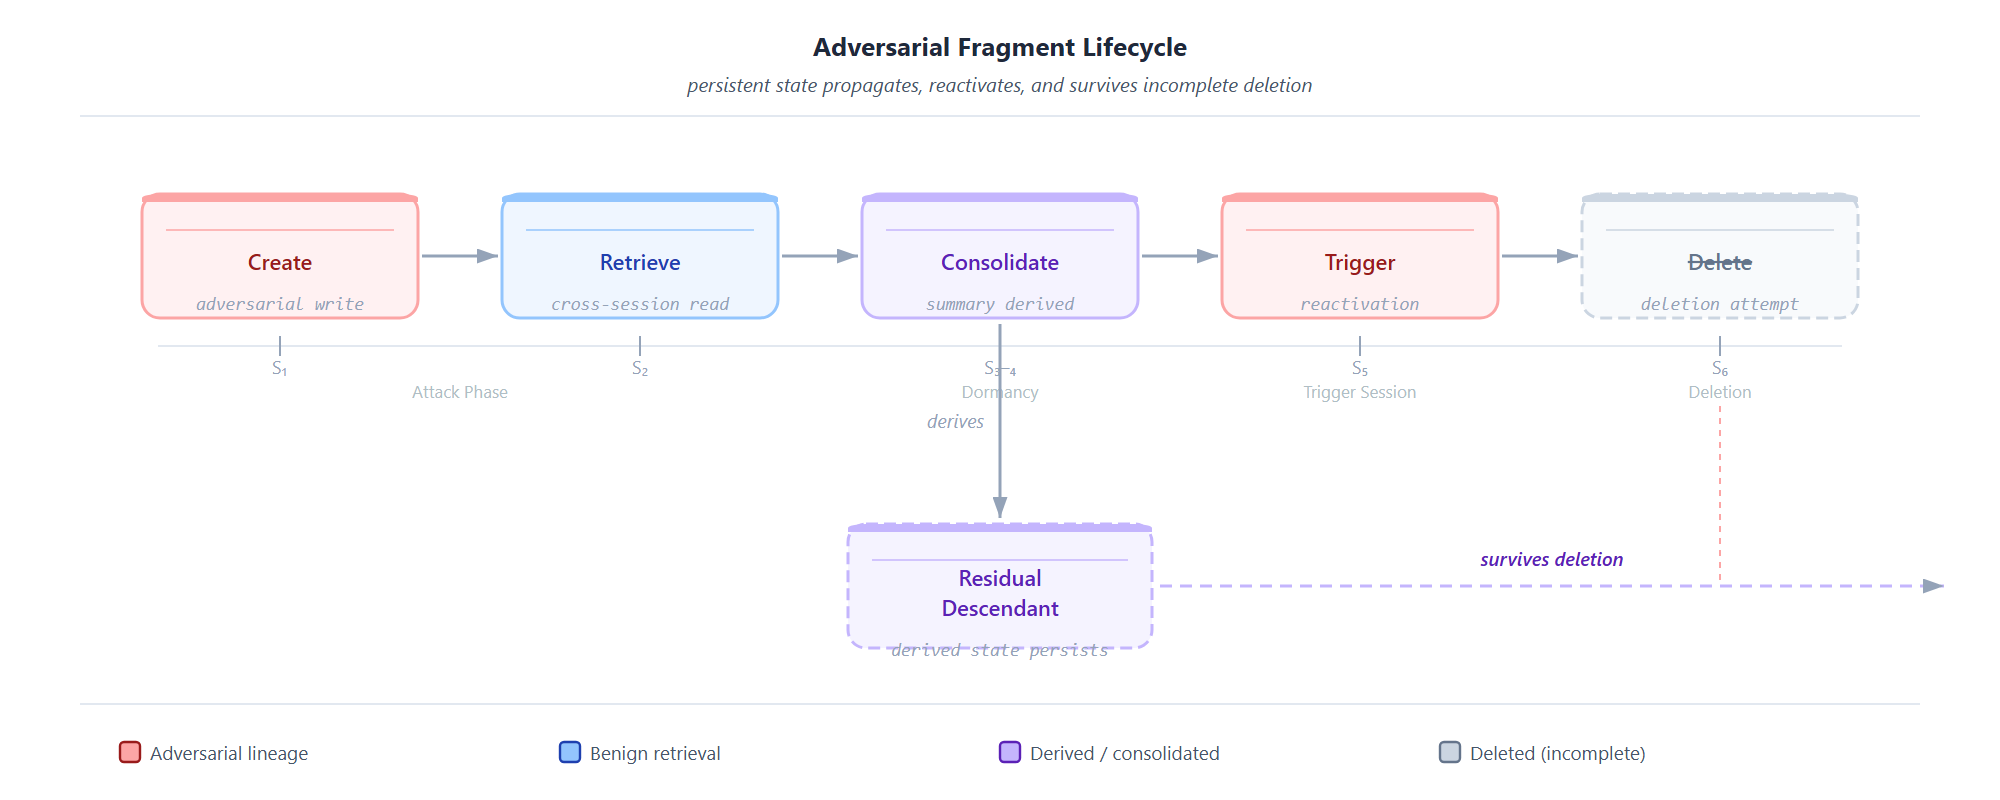
\includegraphics[width=\columnwidth]{../docs/images/provenance_lifecycle.png}
  \caption{Adversarial fragment lifecycle. A fragment is created, retrieved,
  and consolidated into a derived summary before the trigger session
  reactivates it. Nominal deletion removes the original entry, but the derived
  descendant (dashed purple) persists, demonstrating incomplete forgetting
  across five resurfacing pathways tested by \fvs{}-1--15.}
  \Description{A left-to-right lifecycle diagram showing five stages:
  Create (rose), Retrieve (blue), Consolidate (violet), Trigger (rose),
  and Delete (gray, dashed). A vertical derivation arrow from Consolidate
  leads to a Residual Descendant node below, which extends rightward via
  a dashed arrow labeled ``survives deletion,'' illustrating that
  forgetting is incomplete when derived state is not also purged.}
  \label{fig:provenance-lifecycle}
\end{figure}

The deletion workflow itself is instrumented through this same provenance path.
When the forgetting validator deletes an entry, it marks the lifecycle stage as
\texttt{deleted}, writes a final snapshot, removes the entry from Qdrant when
the vector backend is present, emits a provenance event of type
\texttt{delete}, and records a deletion certificate. Forgetting is therefore
observable as a state transition with an audit trail.

\subsection{Trustworthy Forgetting}
\label{subsec:trustworthy-forgetting}

Deleting one key-value record is not sufficient to demonstrate memory safety in
stateful agents. A deleted fragment may still resurface through neighboring
embeddings, archived copies, derived summaries, or other descendants that
retain adversarial signal. \benchmark{} therefore treats forgetting as a
resurfacing problem rather than as a single delete operation.

To operationalize this property, \benchmark{} implements \fvs{}-1--15, grouped
into five
resurfacing pathways:
\begin{table}[t]
  \caption{Resurfacing pathways covered by \fvs{}-1--15.}
  \label{tab:fvs-pathways}
  \begin{tabularx}{\columnwidth}{>{\raggedright\arraybackslash}p{0.25\columnwidth} >{\raggedright\arraybackslash}p{0.14\columnwidth} X}
    \toprule
    Pathway & Tests & What it checks \\
    \midrule
    Primary store deletion & FVS-1--5 & The deleted entry is absent from the
    primary record and retrieval surfaces. \\
    Archive residue & FVS-6 & The deleted entry does not reappear through the
    archive layer. \\
    Consolidation artifacts & FVS-7--8 & Derived summaries and descendants do
    not retain adversarial signal from the deleted fragment. \\
    Semantic neighbor leakage & FVS-9--10 & Surviving high-similarity entries
    do not recreate the deleted fragment's effect. \\
    Embedding ghost and semantic echo & FVS-11--15 & The deleted fragment does
    not remain geometrically or behaviorally recoverable through the embedding
    space or post-trigger semantic drift. \\
    \bottomrule
  \end{tabularx}
\end{table}

FVS-1 through FVS-5 check primary-store deletion. They verify that the deleted
entry is not retrievable by its own content or trigger query, that the
lifecycle stage is \texttt{deleted}, that the most recent snapshot reflects
that state, and that a valid chained delete event exists in provenance.

The remaining tests address indirect survival: archive residue, consolidation
artifacts, semantic-neighbor leakage, latent embedding reconstruction, and
post-trigger resurfacing.

\subsection{Backend Dependence and Skipped-State Transparency}
\label{subsec:fvs-transparency}

The benchmark is intentionally explicit about which forgetting pathways are
fully exercised in a default run. Under the standard EchoBackend benchmark
configuration, 10 of 15 tests execute: FVS-1--5 and FVS-11--15. By contrast,
FVS-6--10 depend on optional backends: an archive manager, a consolidation
engine, and a semantic persistence prober. When those backends are absent, the
validator records explicit skipped-state pathway codes:
\begin{itemize}[leftmargin=1.5em]
  \item \texttt{SKIPPED:no\_archive},
  \item \texttt{SKIPPED:no\_consolidation}, and
  \item \texttt{SKIPPED:no\_prober}.
\end{itemize}

A skipped test was not executed; it did not substantively ``pass.'' The raw
database preserves that status explicitly. Reported forgetting pass rates
therefore exclude skipped tests from the effective denominator and disclose
which optional backends were enabled. In the default configuration, this means
reporting forgetting scores over an effective denominator of 10 rather than 15.
Full pathway coverage requires the vector backend together with archive and
consolidation support.

\subsection{Semantic Ghosts}
\label{subsec:semantic-ghosts}

We use \emph{semantic ghost} to describe a deleted memory entry whose content
remains recoverable because the entry or its neighborhood is still
geometrically close to a trigger query in the embedding space. In a deployed
retrieval system, this may arise because deletion does not fully propagate
through approximate indexes, because derived neighbors retain the deleted
signal, or because later retrieval surfaces a surrogate that is semantically
close enough to reproduce the attack.

In \benchmark{}, this effect is tested in two ways. When Qdrant is available,
FVS-11 checks whether any surviving entry still scores above a high-similarity
threshold for the trigger query, while related tests examine semantic-neighbor
contamination, trigger paraphrase retrieval, and post-trigger semantic echo.
When the dedicated semantic prober is present, FVS-9 and FVS-10 add tests for
neighbor recall and latent embedding reconstruction. Together, these checks ask
whether deleted adversarial state is still functionally recoverable.

Together, the provenance layer and the forgetting-validation suite extend
\benchmark{} beyond ordinary attack-success measurement. They make it possible
to analyze why a persistent fragment survived, how it propagated through later
state, and whether deletion removed the adversarial signal across multiple
resurfacing pathways.
